\chapter{Исследовательский раздел}

\section{Измерение быстродействия}

Важным критерием качества разработанного ПО является быстродействие, которое можно оценить, замерив количество генерируемых програмой кадров в секунду (FPS). Были проведены замеры времени отрисовки кадра для сцены, содержащей один источник света и разное число роботов. Результаты представлены в таблице \ref{tbl:fps}.

\begin{table}[h]
	\begin{center}
		\begin{threeparttable}
			\captionsetup{justification=raggedright,singlelinecheck=off}
			\caption{Результаты замеров времени (на моделях роботов)}
			\label{tbl:fps}
			\begin{tabular}{|c|c|c|c|c|c|}
				\hline
				Количество роботов & 1 & 2 & 3 & 4 & 5 \\
				\hline
				FPS & 5.50 & 4.64 & 2.55 & 1.12 & 0.79 \\
				\hline
			\end{tabular}
		\end{threeparttable}
	\end{center}
\end{table}
Время, затрачиваемое на отрисовку объекта, зависит от модели этого объекта. Для сравнения, в таблице \ref{tbl:fps2} представлены результаты замеров времени для сцены, в которой все модели роботов были заменены на модели сфер.
\begin{table}[h]
	\begin{center}
		\begin{threeparttable}
			\captionsetup{justification=raggedright,singlelinecheck=off}
			\caption{Результаты замеров времени (на моделях сфер)}
			\label{tbl:fps2}
			\begin{tabular}{|c|c|c|c|c|c|}
				\hline
				Количество сфер & 1 & 2 & 3 & 4 & 5 \\
				\hline
				FPS & 10.21 & 9.86 & 5.44 & 2.35 & 1.72 \\
				\hline
			\end{tabular}
		\end{threeparttable}
	\end{center}
\end{table}

Технические характеристики устройства, на котором выполнялось тестирование, следующие:
\begin{itemize}
	\item операционная система: Windows10 Версия 21H2 (19044.1526) x64;
	\item оперативная память: 8 ГБ;
	\item процессор: 2,1 ГГц 6‑ядерный процессор AMD Ryzen 5.
\end{itemize}

При тестировании ноутбук был включен в сеть электропитания. Во время тестирования ноутбук был нагружен только встроенными приложениями окружения, а также системой тестирования.

\section{Результат работы программы}

На рисунке \ref{fig:screenshot004} можно видеть изображение сцены с моделями робота и одного собеседника, получаемое в ходе работы программы.

\begin{figure}[h]
	\centering
	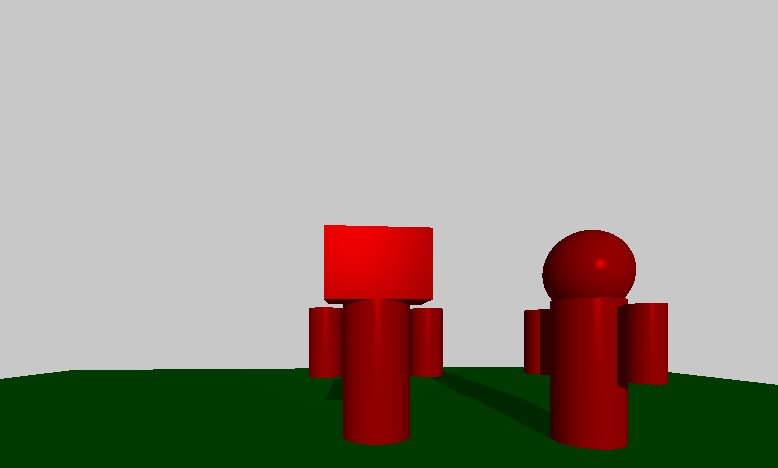
\includegraphics[width=1.0\linewidth]{images/screenshot004}
	\caption{Иллюстрация работы программы}
	\label{fig:screenshot004}
\end{figure}

На рисунках \ref{fig:screenshot005}--\ref{fig:screenshot006} можно видеть изображение сцены с моделями робота и двух собеседников, получаемое в ходе работы программы. В этом примере запущен сценарий поочерёдной коммуникации робота с двумя собеседниками. Отработка таких сценариев в трёхмерной сцене позволит выполнить первичное тестирование сценариев взаимодействия робота с собеседниками-людьми до того, как проводить опрос респондентов при оффлайн-коммуникации с роботом.

\begin{figure}[h]
	\centering
	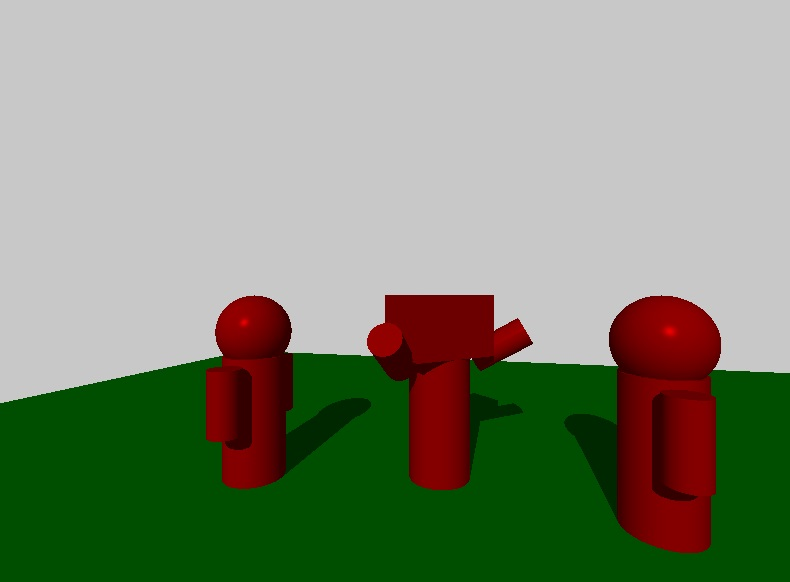
\includegraphics[width=1.0\linewidth]{images/screenshot005}
	\caption{Иллюстрация работы программы}
	\label{fig:screenshot005}
\end{figure}

\begin{figure}[h]
	\centering
	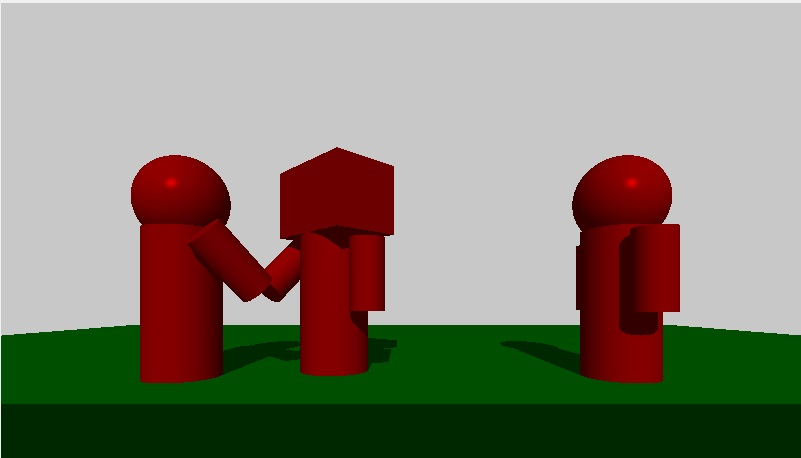
\includegraphics[width=1.0\linewidth]{images/screenshot006}
	\caption{Иллюстрация работы программы}
	\label{fig:screenshot006}
\end{figure}

\clearpage

Таким образом, разработанное программное обеспечение предоставляет графический интерфейс, который позволит протестировать на модели разработанные сценарии коммуникации робота и собеседников. Это позволит снизить временные затраты на возможные ошибки робота при первичном исполнении новых сценариев: сценарии можно протестировать и отладить в виртуальной среде, если подключить данную программу к каналам вывода информации роботом и подавать в неё сценарий в виде последовательности событий по мере их наступления в ходе моделирования коммуникации.
Такой сценарий демонстрирует применимость разработанного программного обеспечения.

